\documentclass{article}
\usepackage{xeCJK}
\usepackage{amsmath}
\usepackage{listings}
\usepackage{xcolor}
\setlength{\parindent}{0pt}
\renewcommand{\baselinestretch}{1.0}
\lstset{
	frame=tb, % draw a frame at the top and bottom of the code block
	showstringspaces=false, % don't mark spaces in strings
	numbers=left, % display line numbers on the left
	commentstyle=\color{green}, % comment color
	keywordstyle=\color{blue}, % keyword color
	stringstyle=\color{red} % string color
}
\usepackage[a4paper,left=20mm,right=20mm,top=15mm,bottom=15mm]{geometry}  

\title{Extend KMP}
\author{MengChunlei}

\begin{document}
\maketitle
\section{算法目标}
给定字符串S和T,长度分别为$n,m$.用$SubS(i,j), SubT(i,j)$表示S,T的子串.计算一个长度为$n$的数组$e$.其中$e[i]$表示$SubS(i,n-1)$和T的最长公共前缀. \par
可以看出, 如果$e[i]=m$,那么说明S包含T.所以这个算法是kmp算法的扩展.

\section{算法描述}
这个算法依赖于在T上的一个辅助数组$f$,其中$f[i]$表示$SubT(i,m-1)$和T的最长公共前缀.假设现在已经计算出了$f$. \par
另外, 这个算法是递进的.也就是说, $e[i]$的计算依赖于$e[0],e[1],...,e[i-1]$.所以, 现在假设已经计算出了$e[0],e[1],...,e[i-1]$. \par
这里定义两个数字 $a,p$.其中$p=max\ \sum_{k=0}^{i-1}(k+e[k])$, $a$为使得$p$取最大值时对应的$k$. \par
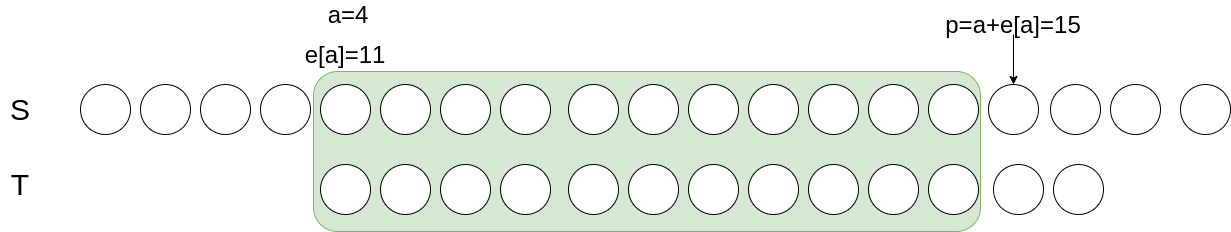
\includegraphics[scale=0.39]{pic1.png} \par
如上图所示, 绿色的上下两部分是相等的.下面考虑$e[i]$. \par
第一种情况, $i+f[i-a]<p$. 如下图, $f[i-a]=3$.其中$t=f[i-a]$ \par
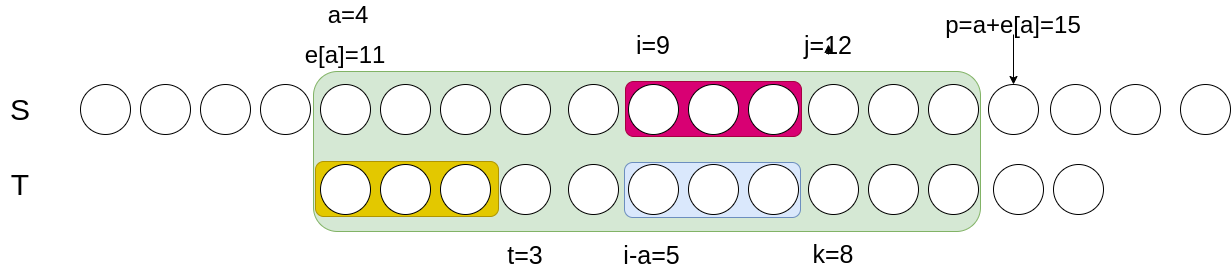
\includegraphics[scale=0.39]{pic2.png} \par
那么由上图可以知道,蓝色的跟黄色的相等, 蓝色的跟红色的相等, 所以黄色的跟红色的相等. 并且, 由于$f[i-a]=3$, 所以$T[t]\neq T[k]$, 但是$T[k]=S[j]$, 所以$T[t] \neq S[j]$, 所以$e[i]=f[i-a]=3$.\par
~\\
第二种情况,$i+f[i-a]=p$. 如下图,$f[i-a]=6$ \par
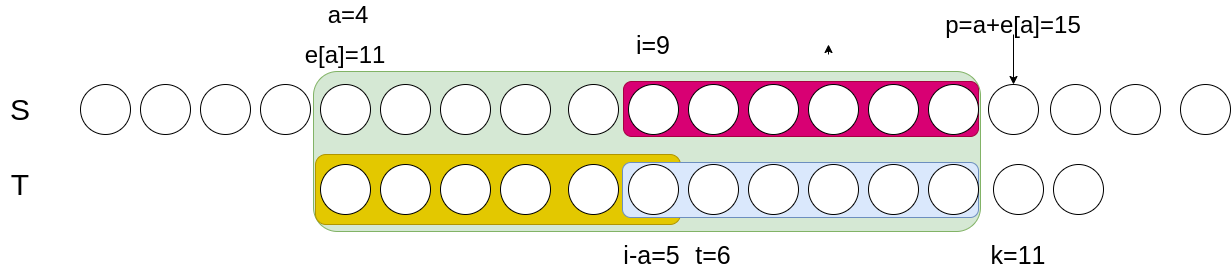
\includegraphics[scale=0.39]{pic3.png} \par
那么由上图可以知道,蓝色的跟黄色的相等, 蓝色的跟红色的相等, 所以黄色的跟红色的相等. 并且, 由于$f[i-a]=6$, 所以$T[t]\neq T[k]$, 同时$T[k]\neq S[p]$, 所以$T[t]$有可能等于$S[p]$, 所以这个时候需要向后比较, 直到找到一个位置$x$满足$S[x]$不等于对应的T的字符,那么此时$e[i]=x-i$. 并且这时候应该更新$p,a$为$p=x,a=i$.\par
~\\
第三种情况,$i+f[i-a]>p$. 如下图,$f[i-a]=8$ \par
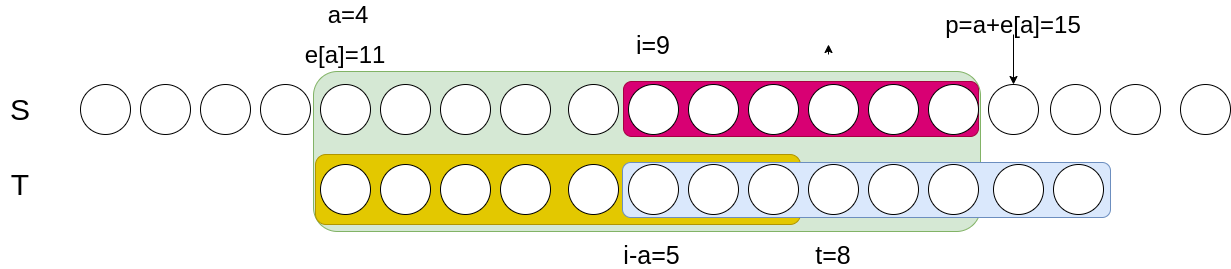
\includegraphics[scale=0.39]{pic4.png} \par
这种情况导致的结果跟第二种情况一样, 需要从$S[p]$开始, 跟$T$对应的字符依次开始比较, 直到找到一个不等的位置, 然后同样要更新$p,a$.
~\\
下面给出计算$e$的代码.
\begin{lstlisting}[language=C++, caption={Compute array $e$}]
std::vector<size_t> GetE(const std::string &S, const std::string &T,
                         const std::vector<size_t> &f) {
  const size_t n = S.size();
  const size_t m = T.size();
  std::vector<size_t> e(n);
  size_t a = 0, p = 0;
  for (size_t i = 0; i < n; ++i) {
    if (i >= p || i + f[i - a] >= p) {
      if (i > p) {
        p = i;
      }
      while (p < n && p - i < m && S[p] == T[p - i]) {
        ++p;
      }
      e[i] = p - i;
      a = i;
    } else {
      e[i] = f[i - a];
    }
  }
  return e;
}
\end{lstlisting}

\section{$f$的计算}
来看下$f$和$e$的区别 \par
i $f[i]$表示 $SubT(i,m-1)$和T的最长公共前缀 \par
ii $e[i]$表示 $SubS(i,n-1)$和T的最长公共前缀 \par
所以$f$的计算方法跟$e$类似. 下面是计算$f$的代码. \par
\begin{lstlisting}[language=C++, caption={Compute array $f$}]
std::vector<size_t> GetF(const std::string &T) {
  const size_t m = T.size();
  std::vector<size_t> f(m, m);
  size_t a = 0, p = 0;
  for (size_t i = 1; i < m; ++i) {
    if (i >= p || i + f[i - a] >= p) {
      if (i > p) {
        p = i;
      }
      while (p < m && T[p] == T[p - i]) {
        ++p;
      }
      f[i] = p - i;
      a = i;
    } else {
      f[i] = f[i - a];
    }
  }
  return f;
}
\end{lstlisting}


\end{document}
